% !TEX root = ../main.tex

%************************************************
\chapter{Conclusions / Future Work}
\label{ch:conclusions} 

%************************************************

We have explored relationships between BLR outflows, NLR outflows and hot dust emission. 

Put some stuff from research proposals here 

\section{Future: Red quasars}

Punctuated fuelling episodes, e.g. driven by galaxy mergers, satellite accretion and even secular processes,
almost certainly lead to AGN experiencing activity-, outflow- and obscuration-dominated cycles with some overlap between phases. 
However, quantitatively, it remains unclear how these phases relate to the fundamental properties of the accreting black-hole (e.g.  mass (M$_{\mathrm{BH}}$), bolometric luminosity (L$_{\mathrm{bol}}$) and Eddington ratio (L/L$_{\mathrm{Edd}}$) and the elements of the non-spherical geometry).


% \section{Future work}
% \todo{To do}
% \begin{itemize}
% \item Publish definitive masses using Allen \& Hewett redshifts 
% \item See Park criticism (low blueshift end)
% \item Data-driven mapping - see research proposal and Joe's email.
% \end{itemize}

% Allen \& Hewett will publish improved redshifts for all quasars in the SDSS DR$7$ and DR$12$ catalogues. 
% At the same time we will publish catalogues of unbiased BH masses for both SDSS DR$7$ and DR$12$ based on the Allen \& Hewett redshifts. 
% The components from the mean-field independent component analysis \citep[see][for an application to astronomical spectra]{allen13} used in the Allen \& Hewett redshift algorithm will also be published.
% With these components, if a rest-frame ultraviolet spectrum is available, it will be straightforward to determine the systemic redshift, via a simple optimisation procedure, and hence calculate the \ion{C}{IV} blueshift. 

% Large scatter remains, particularly at low \ion{C}{IV} blueshifts. 
% Some of this is correlated with the \ha FWHM, which is in turn correlated with EV1. 
% However, no good - need something in the UV spectrum. 
% Remarkable we can do so well with a single parameter, but try Blueshift+EQW (e.g. Runnoe)
% But better to use data-driven approach (see research proposal stuff). 

% Mention John's clustering work. 

% Conversely, there are no quasars in our catalogue with \ion{C}{IV} blueshifts $\lesssim0$\,\kms\, and we caution against extrapolating the correction formula to negative blueshifts.
% In particular, quasars with negative blueshifts as large as $\sim1000$\,\kms appear in the SDSS DR$7$ catalogue and applying our correction in this regime boosts the derived masses by unphysical factors.    
% Need more low blueshift quasars
% Hints of tension so then proabbly need a mroe flexbible model

\noindent My research has focused on measuring fundamental properties of quasars and quasar-driven outflows in large surveys, with the ultimate goal of understanding the crucial role played by quasars in the evolution of galaxies.
Building on this experience, I plan to (1) use data-driven methods to maximise the information content of spectroscopic survey data, (2) study galaxy-wide outflows traced by narrow [\ion{O}{III}] emission, (3) use integral field unit (IFU) spectroscopy to measure the morphology and energetics of these outflows and their effect on star formation, and (4) use multi-wavelength spectral energy distribution (SED) modelling to study how these outflows are powered.  
My proposed projects, which are summarised below, would mesh effectively with the Galaxy Evolution and SAMI research programs. 

In \citet{coatman17}, I derived a direct empirical correction that maps the \ion{C}{IV} line-width and blueshift (relative to the quasar rest-frame) to the Balmer emission-based black hole (BH) mass. 
I plan to extend this by developing a purely data-driven approach to inferring the BH mass from the rest-frame UV spectrum. 
Allen \& Hewett (in preparation) have run an independent component analysis (ICA) on the SDSS quasar sample that compresses all of the information contained in the UV spectra into a small number of component weights.
Taking the set of 230 objects with NIR spectra (and hence reliable Balmer-based BH masses), I will build a model that learns how these ICA component weights depend on the BH mass. 
After the training step, I can use the model to predict a BH mass (and the associated uncertainty) based only on the ICA component weights for the UV spectrum.
There are numerous algorithms available to tackle this class of supervised learning problem (e.g. random forests). 

Taking this one step further, I will build a data-driven model that predicts the unseen rest-frame optical spectrum from the UV region probed by SDSS spectra at redshifts $z\gtrsim2$.
This approach is inspired by the data-driven model for deriving stellar labels from spectroscopic data developed by \citet{ness15}.
I will use an ICA to generate a set of `labels' describing the optical spectrum. 
I will build a flexible generative model that predicts the flux at each wavelength in the SDSS rest-frame UV spectrum as a function of these weights.
The coefficients in this model, which could be linear or a low-order polynomial, will be trained on the sub-sample of quasars with spectra covering the full optical to UV region. 
Once the coefficents have been determined, I will be able to statistically infer the optical ICA component weights based only on the UV spectrum. 
The optical spectrum can then straightforwardly be reconstructed from the ICA component weights and parameters of interest, such as the BH mass, can be calculated, without the need for follow-up NIR spectroscopy. 
I will also investigate whether an ICA decomposition (or any dimensionality reduction algorithm) can be used to infer the intrinsic quasar luminosity. 
The uncertainty on a single measurement would certainly be large but, with spectra for hundreds of thousands of quasars out to high redshifts, quasars could be used as standard candles to constrain cosmological parameters. 
I am keen to apply similar techniques to other spectroscopic surveys in which CAASTRO researchers are involved. 





% \begin{wrapfigure}{}{0.5\textwidth}
% \centering
% 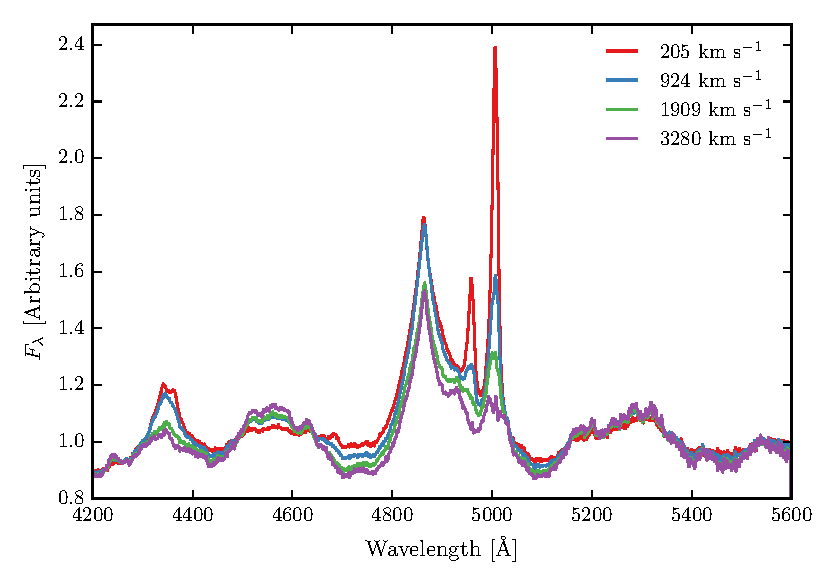
\includegraphics[width=0.5\textwidth]{mfica_composites.pdf}
% \caption{[\ion{O}{III}] becomes weaker and more blueshifted as the \ion{C}{IV} blueshift increases (Coatman et al., 2017b, in prep.).}
% \label{fig:mfica_composites}
% \end{wrapfigure}

\section{Studying feedback with IFU spectroscopy}

Unfortunately, integrated spectra contain little information on the spatial extent or geometry of the outflowing gas.  
To study the morphology and energetics of the outflow, we must turn to spatially-resolved IFU spectroscopy.
IFU spectroscopy has revealed outflowing ionised gas on scales of $\sim10$kpc to be common in the hosts of quasars at low redshifts \citep[e.g.][]{harrison14}. 
Extended outflows have also been detected at high redshifts ($z\gtrsim2$) in a handful of objects \citep[e.g.][]{carniani15}. 

Currently, I am analysing the spatially-resolved kinematics of the ionised gas in the hosts of $\sim$120 luminous quasars at redshifts $z\sim2$ using (mostly archival) SINFONI IFU spectra. 
I have already analysed the spatially-integrated spectra and in many a broad, blueshifted wing in the [\ion{O}{III}] emission is clearly identifiable. 
An ICA on a sample of low-redshift SDSS quasar spectra has been used to generate individual components corresponding to the [\ion{O}{III}] emission originating in static and outflowing gas. 
I can use the relative weights of these two components in each spaxel to generate velocity maps and compare the spatial distributions of the static and outflowing components.
I can then test whether the outflowing component in the [\ion{O}{III}] emission extends to $\sim$kpc scales and
estimate properties of the ionised outflows: the mass outflow rate, momentum rate, and kinetic power.
I will also search for narrow \ha emission associated with star formation, using the relative strength of [\ion{N}{II}] to discriminate between a star formation and AGN origin of the narrow \ha emission \citep{susie16}. 
I will look for anti-correlations in the spatial distributions of outflowing gas and star forming regions, which would be indicative of negative quasar feedback in action.

These observations will be challenging and, given the limited depth of our data, the [\ion{O}{III}] emission is unlikely to be spatially resolved in every object. 
Therefore, I would like to observe a representative sub-set of the large sample presented in Coatman et al. (2017b, in prep.) using SINFONI or KMOS on the VLT. 
Because I have already carefully analysed the [\ion{O}{III}] emission properties of these quasars, it is an ideal sample from which to select targets for IFU spectroscopy. 
One particular goal is to understand the disappearance of the narrow line region in quasars with strong broad line region outflows (Fig.~\ref{fig:mfica_composites}). 

The majority of the un-obscured quasars in this sample lack optical spectra. 
Therefore, to exploit the rich information contained in the rest-frame UV spectrum (e.g. the BLR outflow properties) I propose to observe these targets. 
The sample is relative bright ($b_J\sim17.5$) and so this could easily be achieved on a moderately-sized telescope. 
I will then be able to extend my study of the relationship between outflows in the broad and narrow line regions. 


More careful modelling of \ion{Fe}{II} emission with different tempaltes or cloudy models. 
 Recommends instead taking the line ratios in some paper, and broadening the spectra to make a grid. Sherpa allows you to interpolate over the grid of templates in the fit. 


\section{Future prospects}

